\documentclass[12pt, letterpaper]{article}
\usepackage{graphicx} % Required for inserting images
\usepackage{amsmath}
\usepackage{mdframed}

\title{telegraph equations solved with MFEM library}
\author{Denis Lachapelle}
\date{February 2025}

\setlength{\parindent}{0pt}

\begin{document}

\maketitle

\section{Introduction}
This document explains the telegraph equations simulation using finite differences method based on MFEM library.


\section{Theory, Finite Differences}

The telegraph equations are:

\begin{equation}\frac{\partial{V}}{\partial{x}} + L \frac{\partial{I}}{\partial{t}} + R I = 0\end{equation}


\begin{equation}\frac{\partial{I}}{\partial{x}} + C \frac{\partial{V}}{\partial{t}} + G V = 0\end{equation}


\begin{enumerate}
\item Assume the TL is divided in N segments with node 0 to N. There is N+1 nodes. So nodes are located at $n \Delta x$.
\item Time is sampled at $k \Delta T$.
\item Assume the $\frac{\partial V(t, x)}{\partial x}$ and $\frac{\partial I(t, x)}{\partial x}$ are constant over each segment.
\end{enumerate}

So at a given time $k \Delta T$ we can express the $\frac{\partial V(t, x)}{\partial x}$ and $\frac{\partial I(t, x)}{\partial x}$ as difference  $\frac{V(k \Delta T, (n+1) \Delta x) - V(k \Delta T, (n-1) \Delta x)}{2 \Delta x}$ and  $\frac{I(k \Delta T, (n+1) \Delta x) - I(k \Delta T, (n-1) \Delta x)}{2 \Delta x}$.\\

with the $\frac{\partial}{\partial t}$ on the left side.

\begin{equation} \frac{\partial{I}}{\partial{t}} = - \frac{R I}{L} - \frac{1}{L} \frac{\partial{V}}{\partial{x}} \end{equation}


\begin{equation} \frac{\partial{V}}{\partial{t}} = -\frac{G V}{C} - \frac{1}{C} \frac{\partial{I}}{\partial{x}}\end{equation}




We can write matrix equations....

\begin{equation}
\frac{\partial{I}}{\partial{t}} 
=
	\begin{bmatrix}
		Dv & Ri
	\end{bmatrix}
	\begin{bmatrix}
		V^k \\
		I^k \\
	\end{bmatrix}
\end{equation}

\begin{equation}
	\frac{\partial{V}}{\partial{t}} 
	=
	\begin{bmatrix}
		Gv & Di
	\end{bmatrix}
	\begin{bmatrix}
		V^k \\
		I^k \\
	\end{bmatrix}
\end{equation}

The two equations above can be written as a single matrix equation...

\begin{equation}
    \begin{bmatrix}
    	\frac{\partial{V}}{\partial{t}} \\
    	\frac{\partial{I}}{\partial{t}} 
    \end{bmatrix}	
	=
	\begin{bmatrix}
		Gv Di \\
		Dv Ri
	\end{bmatrix}
	\begin{bmatrix}
		V^k \\
		I^k \\
	\end{bmatrix}
\end{equation}


Where Dv and Di are the same derivative matrix multiplied by different terms -1/L for Dv and -1/C for Di.

\begin{equation}
	\begin{bmatrix}
	   0 & -1/2h & 0 & 0 & ... &0 &0 \\
	   1/2h & 0 &-1/2h & 0 & 0 &... &0 \\
	   0& 1/2h & 0 &-1/2h & 0 &... &0 \\
	   0& 0& 01/2h & 0 &-1/2h & ... &0 \\
	   0& 0& 0&... 1/2h & 0 &-1/2h &0  \\
	   0& 0& 0&... & 1/2h & 0 & 1/2h  \\
	   0& 0& 0& 0&... & 1/2h & 0  \\
	\end{bmatrix}
\end{equation}

Gv and Ri are identity matrix scale by either -G/C and -R/L.

For Dv the multiplier value will be $\frac{\Delta t}{L h}$.

Using the above operator we will step in time using RK4.



\begin{equation}
	\begin{bmatrix}
		V^{k+1} \\
		I^{k+1} \\
	\end{bmatrix}
	=
	\begin{bmatrix}
		V^k \\
		I^k \\
	\end{bmatrix}
	+
	\Delta t
	\begin{bmatrix}
		\frac{\partial{V}}{\partial{t}} \\
		\frac{\partial{I}}{\partial{t}} 
	\end{bmatrix}	
\end{equation}

\begin{equation}
	\begin{bmatrix}
		V^{k+1} \\
		I^{k+1} \\
	\end{bmatrix}
	=
	\begin{bmatrix}
		V^k \\
		I^k \\
	\end{bmatrix}
	+
	\Delta t
	\begin{bmatrix}
		Gv Di \\
		Dv Ri
	\end{bmatrix}
	\begin{bmatrix}
		V^k \\
		I^k \\
	\end{bmatrix}	
\end{equation}


\subsection{MFEM Implementation}

The program is named stltfdrk4.cpp for Single Transmission Line Transient Finite Difference runge kutta 4.

The signal injected is  gaussian pulse centered at 100ns with a Tau of 20ns multiplied by a triangular window of 200ns wide centered at 100ns.\\

\begin{figure}[h]
	\centering
	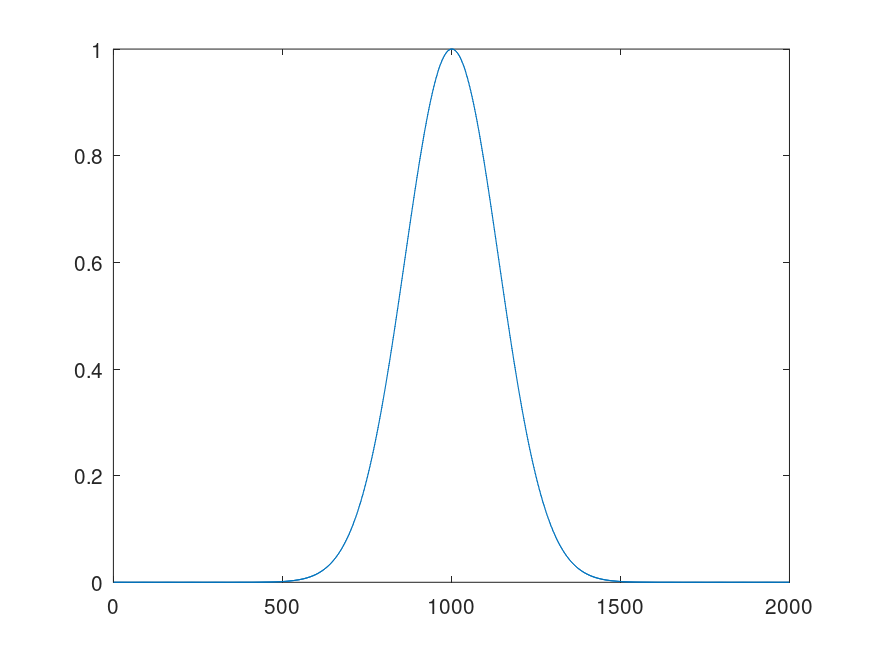
\includegraphics[width=0.8\textwidth]{gaussian_pulse.png} % Adjust width as needed
	\caption{Test pulse}
	\label{fig:example}
\end{figure}

next step is the time step...


\end{document}
